\let\negmedspace\undefined
\let\negthickspace\undefined
\documentclass[journal]{IEEEtran}
\usepackage[a5paper, margin=10mm, onecolumn]{geometry}
%\usepackage{lmodern} % Ensure lmodern is loaded for pdflatex
\usepackage{tfrupee} % Include tfrupee package

\setlength{\headheight}{1cm} % Set the height of the header box
\setlength{\headsep}{0mm}     % Set the distance between the header box and the top of the text

\usepackage{gvv-book}
\usepackage{gvv}
\usepackage{cite}
\usepackage{amsmath,amssymb,amsfonts,amsthm}
\usepackage{algorithmic}
\usepackage{graphicx}
\usepackage{textcomp}
\usepackage{xcolor}
\usepackage{txfonts}
\usepackage{listings}
\usepackage{enumitem}
\usepackage{mathtools}
\usepackage{gensymb}
\usepackage{comment}
\usepackage[breaklinks=true]{hyperref}
\usepackage{tkz-euclide} 
\usepackage{listings}
% \usepackage{gvv}                                        
\def\inputGnumericTable{}                                 
\usepackage[latin1]{inputenc}                                
\usepackage{color}                                            
\usepackage{array}                                            
\usepackage{longtable}                                       
\usepackage{calc}                                             
\usepackage{multirow}                                         
\usepackage{hhline}                                           
\usepackage{ifthen}                                           
\usepackage{lscape}
\begin{document}

\bibliographystyle{IEEEtran}
\vspace{3cm}

\title{1.6.15}
\author{EE25BTECH11065 - Yoshita}
% \maketitle
% \newpage
% \bigskip
{\let\newpage\relax\maketitle}

\renewcommand{\thefigure}{\theenumi}
\renewcommand{\thetable}{\theenumi}
\setlength{\intextsep}{10pt} % Space between text and floats
\textbf{Question}:\\
    Find the value of m if the points $\vec(5,1)$, $\vec(-2,-3)$ and $\vec(8,2m)$ are collinear.\\
\bigskip

\textbf{Solution}:\\
  Let $\vec{A}(5,1)$, $\vec{B}(-2,-3)$, $\vec{C}(8,2m)$.
\\
\begin{table}[H]    
  \centering
  

  \caption{Answers}
  \label{Answers}
\end{table}
Using the collinearity $\brak{rank}$ test, form the matrix with difference vectors:
\begin{align*}
    (\vec{B}-\vec{A} \quad \vec{C}-\vec{A}) &= \myvec{-2-5 & 8-5 \\ -3-1 & 2m-1} \\
    &= \myvec{-7 & 3 \\ -4 & 2m-1}.
\end{align*}
The three points are collinear$\iff$this matrix has rank 1 $\brak{its\ rows\ are\ linearly\ dependent}$.\\
\begin{center}
 $R_2 \leftarrow 7R_2 - 4R_1 \implies  \myvec{-7 & 3 \\ 0 & 14m-19}.$
 \end{center}

For rank $1$, the second row must be zero:
\begin{center}
$14m - 19 = 0 \implies m = \frac{19}{14}$
\end{center}
See Fig. 0 ,
\begin{figure}[H]
\begin{center}
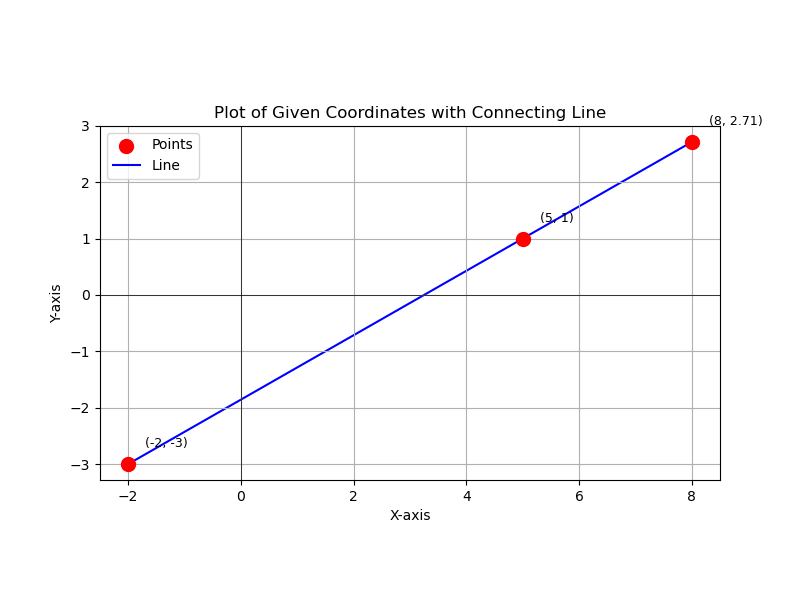
\includegraphics[width=0.6\columnwidth]{figs/fig.png}
\end{center}
\caption{}
\label{fig:Fig.1}
\end{figure}
\end{document}




